
\documentclass[a4paper,12pt]{article}
\usepackage{amsmath,amssymb,graphicx,cite}
\usepackage{hyperref}
\usepackage{geometry}
\geometry{a4paper, margin=1in}

\title{Quantum Work Extraction in a Jaynes-Cummings System with Feedback Control}
\author{Ryan Wallace \\ \texttt{rathmon@gmail.com}}
\date{\today}

\begin{document}

\maketitle

\begin{abstract}
Quantum thermodynamics explores the interplay between quantum mechanics and energy conversion processes. 
This work investigates extractable work (ergotropy) and entanglement in a two-qubit Jaynes-Cummings system 
with an interacting cavity under feedback control. Using the Lindblad master equation, we numerically analyze 
the evolution of concurrence, work extraction, and cavity photon occupation over time. We find that while qubit 
flipping contributes to work extraction, entanglement does not perfectly correlate with available energy, indicating 
the role of nonlocal correlations and cavity-mediated interactions. Our findings have implications for quantum heat 
engines and information-to-energy conversion processes.
\end{abstract}

\section{Introduction}
Quantum thermodynamics seeks to understand energy transfer in small-scale quantum systems where coherence and entanglement 
play a significant role. The Jaynes-Cummings (JC) model \cite{jaynes1963comparison} is a fundamental framework describing 
the interaction between a two-level atom (qubit) and a quantized cavity field, leading to reversible excitation-exchange 
(Rabi oscillations). In this work, we extend the JC model to include feedback control, allowing adaptive modifications 
of the system dynamics based on prior evolution.

A key quantity of interest in quantum thermodynamics is extractable work, quantified by ergotropy \cite{allahverdyan2004maximal}. 
While classical work extraction is determined by thermodynamic gradients, quantum systems enable work extraction from coherence 
and quantum correlations \cite{vinjanampathy2016quantum}. This work aims to explore the role of feedback-induced dynamics in 
modifying extractable work, cavity photon occupation, and qubit entanglement.

\section{Theoretical Framework}

\subsection{Jaynes-Cummings Model with Feedback}
The standard JC Hamiltonian is given by:
\begin{equation}
H_{\text{JC}} = \frac{\hbar \omega_q}{2} \sigma_z + \hbar \omega_c a^\dagger a + \hbar g (\sigma_+ a + \sigma_- a^\dagger),
\end{equation}
where $\omega_q$ and $\omega_c$ are the qubit and cavity frequencies, $g$ is the coupling strength, and 
$a^\dagger (a)$ are the cavity mode creation (annihilation) operators.

To introduce feedback, we modify the system evolution using an adaptive parameter $\beta$, influencing the interaction 
based on previous measurements.

\subsection{Lindblad Master Equation}
To incorporate dissipation and decoherence, we evolve the system using the Lindblad equation:
\begin{equation}
\frac{d\rho}{dt} = -\frac{i}{\hbar} [H, \rho] + \sum_k \gamma_k \left( L_k \rho L_k^\dagger - \frac{1}{2} \{L_k^\dagger L_k, \rho\} \right),
\end{equation}
where $L_k$ are collapse operators representing decay channels (qubit relaxation, cavity loss).

\subsection{Concurrence (Entanglement)}
Entanglement is quantified using concurrence, defined as:
\begin{equation}
C(\rho) = \max(0, \lambda_1 - \lambda_2 - \lambda_3 - \lambda_4),
\end{equation}
where $\lambda_i$ are the eigenvalues of $\sqrt{\sqrt{\rho} \tilde{\rho} \sqrt{\rho}}$, and 
$\tilde{\rho}$ is the spin-flipped density matrix.

\subsection{Extractable Work (Ergotropy)}
The ergotropy of the system is given by:
\begin{equation}
W_{\text{ex}} = \text{Tr}(\rho H) - \min_{U \in \text{SU}(d)} \text{Tr}(U\rho U^\dagger H),
\end{equation}
where the second term accounts for the passive state with the same spectrum as $\rho$ but arranged in decreasing energy order.

\section{Numerical Methods}
We solve the time evolution using the \texttt{solve\_ivp} function from SciPy, discretizing the master equation over time. 
Key observables are computed at each step, including concurrence, ergotropy, and cavity photon occupation.

\section{Results and Discussion}
\subsection{Entanglement Evolution}
\begin{figure}[h]
\centering
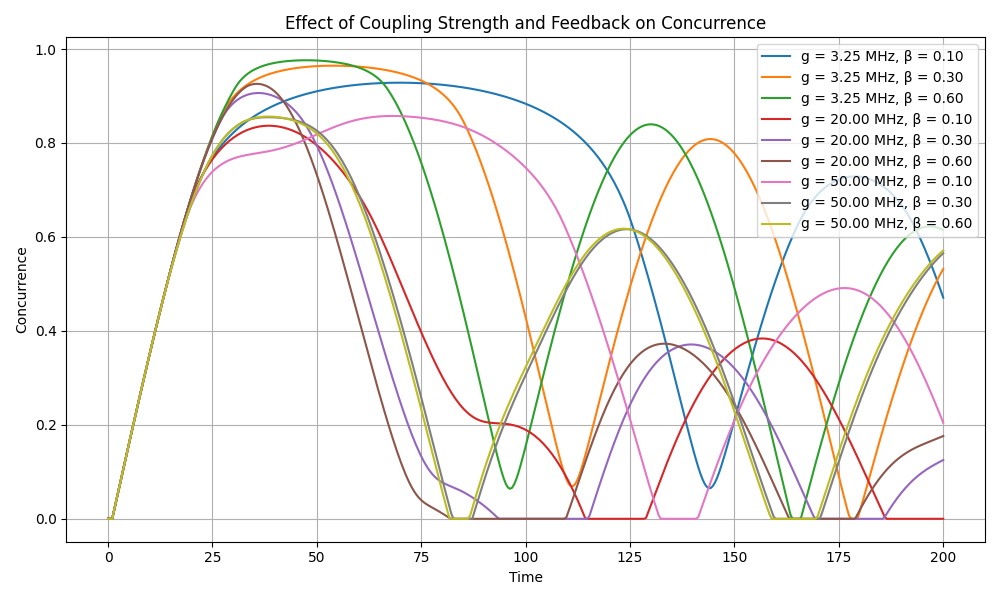
\includegraphics[width=0.7\linewidth]{Figure1.png}
\caption{Time evolution of concurrence for different coupling strengths $g$ and feedback parameters $\beta$.}
\label{fig:concurrence}
\end{figure}

Figure \ref{fig:concurrence} shows the concurrence dynamics over time, demonstrating oscillatory behavior 
dependent on $g$ and $\beta$.

\subsection{Extractable Work Dynamics}
\begin{figure}[h]
\centering
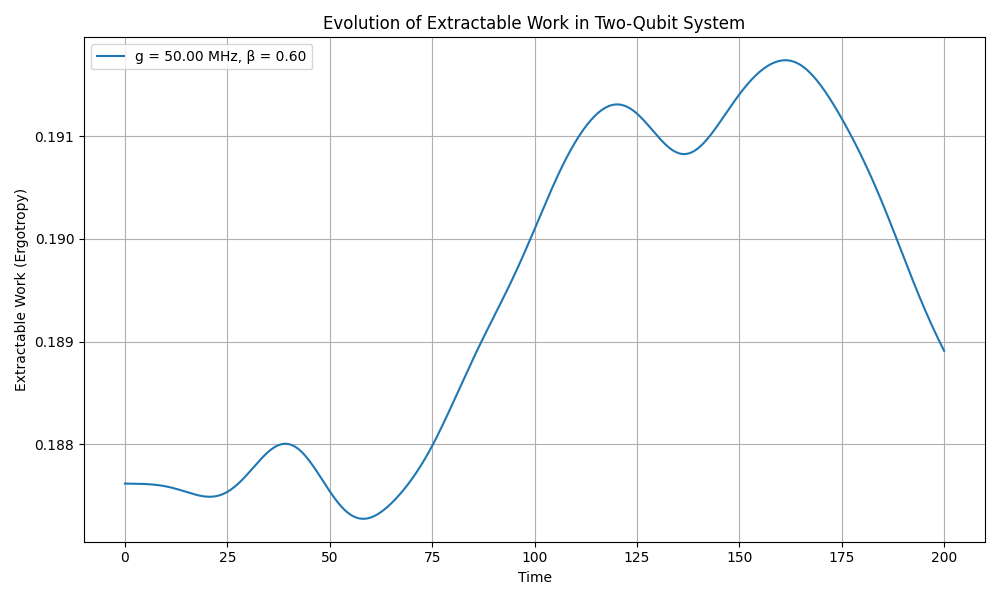
\includegraphics[width=0.7\linewidth]{Figure2.png}
\caption{Extractable work (ergotropy) evolution over time.}
\label{fig:ergotropy}
\end{figure}

Figure \ref{fig:ergotropy} reveals that work extraction does not perfectly align with entanglement, 
suggesting a role for system correlations beyond concurrence.

\subsection{Cavity Photon Occupation}
\begin{figure}[h]
\centering
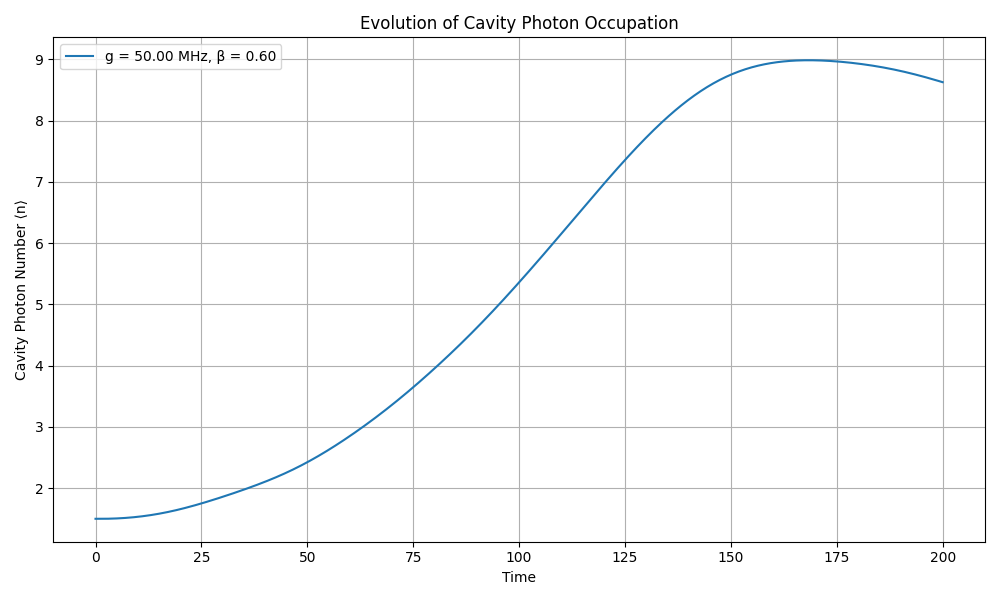
\includegraphics[width=0.7\linewidth]{Figure3.png}
\caption{Evolution of cavity photon occupation.}
\label{fig:photons}
\end{figure}

Photon occupation increases before stabilizing, indicating energy retention in the cavity.

\subsection{Correlation Between Concurrence and Ergotropy}
\begin{figure}[h]
\centering
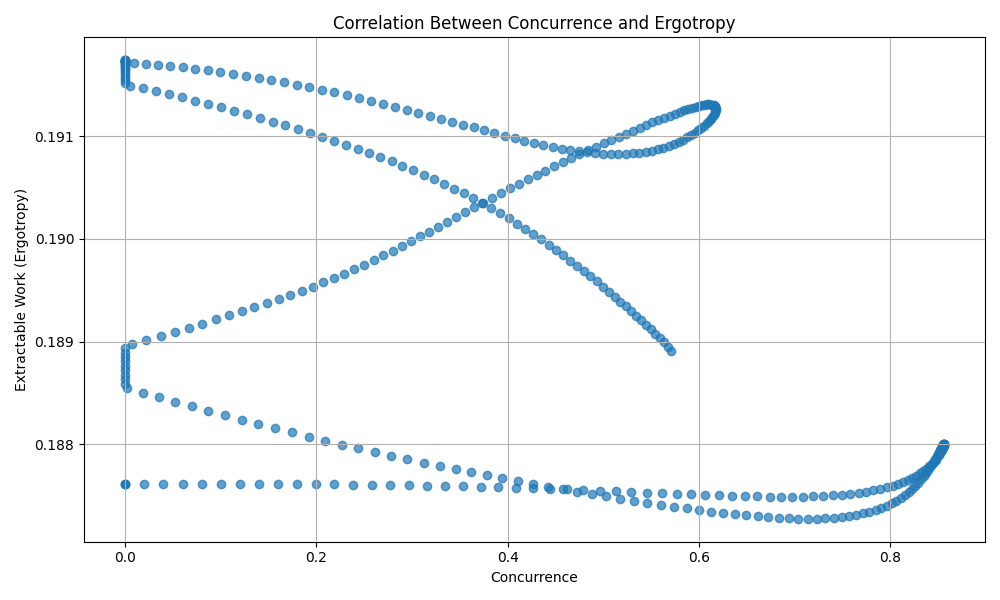
\includegraphics[width=0.7\linewidth]{Figure4.png}
\caption{Correlation between concurrence and extractable work.}
\label{fig:correlation}
\end{figure}

Figure \ref{fig:correlation} highlights the non-trivial relationship between entanglement and work extraction.

\section{Conclusions}
This work demonstrates the interplay of entanglement, work extraction, and cavity dynamics in a feedback-controlled 
Jaynes-Cummings system. While qubit flipping contributes to work extraction, entanglement alone does not fully determine 
available energy, indicating the role of additional system correlations. Future work could explore the impact of mutual 
information and coherence-assisted work extraction.

\begin{thebibliography}{9}
\bibitem{jaynes1963comparison} E. T. Jaynes and F. W. Cummings, ``Comparison of quantum and semiclassical radiation theories with application to the beam maser,'' IEEE Transactions on Information Theory, 1963.
\bibitem{allahverdyan2004maximal} A. E. Allahverdyan et al., ``Maximal work extraction from finite quantum systems,'' EPL, 2004.
\bibitem{vinjanampathy2016quantum} S. Vinjanampathy and J. Anders, ``Quantum thermodynamics,'' Contemporary Physics, 2016.
\end{thebibliography}

\end{document}
